\documentclass[fleqn]{article}

\usepackage[utf8]{inputenc}
\usepackage[russian]{babel}
\usepackage{fullpage}
\usepackage{graphicx}
\usepackage{amsmath}
\usepackage{amsmath,amssymb}
\usepackage{mathbbol}
\usepackage{chngcntr}
\usepackage{hyperref}
\usepackage{tcolorbox}
\DeclareMathOperator{\E}{\mathbb{E}}
\DeclareMathOperator{\V}{\mathbb{Var}}
\DeclareMathOperator{\B}{\mathbb{Bias}}
\counterwithin*{equation}{subsection}
\counterwithin*{equation}{section}

\newcommand\independent{\protect\mathpalette{\protect\independenT}{\perp}}
\newcommand{\indepg}{\perp \!\!\! \perp_G}
\def\define#1{\textbf{def} \textbf{#1}}
\def\independenT#1#2{\mathrel{\rlap{$#1#2$}\mkern2mu{#1#2}}}

\DeclareMathOperator*{\argmin}{argmin} % no space, limits underneath in displays
\DeclareMathOperator*{\argmax}{argmax} % no space, limits underneath in displays

\begin{document}

\section*{Интро}
Заметки по ходу чтения книги Judea Pearl "Causality models, reasoning and inference".

\section*{Introduction to Probabilities, Graphs, and Causal Models}

Какова вообще связь причинности и теории вероятностей? Есть две причины.

Первая состоит в том, что утверждения о причинах и следствиях обычно сопровождаются той или иной степенью уверенности. Часто причины не делают следствие абсолютно обязательным, а лишь повышают его вероятность.

Вторая (она на самом деле довольно сильно связана с первой) состоит в том, что даже весьма очевидные причинно-следственные связи выполняются не всегда, а \textit{почти всегда}: существует множество мелких деталей, которые сложно учесть. 

Рассмотрим факторизацию распределения $P(x_1,...x_N) = \prod\limits_{n}P(x_n|x_1...x_{n-1})$. 

\define{Марковские родители} случайной переменной $X_n$ - минимальное подмножество переменных $PA_n \subset \{X_1...X_{n-1}\}$ такое, что $P(x_n|pa_n) = P(x_n|x_1..x_{n-1})$.

\define{Байесовская сеть} - DAG, построенный с вершинами-переменными и ребрами, соединяющими вершину с её марковскими родителями (рёбра направлены от родителей к детям).

Можно показать, что при заданном упорядочивании переменных марковские родители для каждой переменной определяется однозначно, если распределение $P(X_1,...X_N)$ строго положительно, то есть любая комбинация переменных имеет вероятность $>0$ (понятное дело, если она не содержит значений переменных, маргинальная вероятность которых = 0). Понятно, что это будет достаточным условием, чтобы были определены условные вероятности $P(x_n|x_1..x_{n-1}) = \frac{P(x_1, ..., x_n)}{P(x_1,..,x_{n-1})}$, так как в этом случае знаменатель не будет нигде обращаться в 0 на области определения $P(x_1,...,x_N)$.


\define{Марковская согласованность (Markov Compatibility)} - говорят что распределение $P$ марковски согласованно с DAG $G$, если оно факторизуемо согласно графу, т.е. $P(x) = \prod\limits_n P(x_n|pa_n)$.

Удобным способом характеризации распределений $P$, согласованных с $G$, является список независимостей, которые в этих распределениях должны быть. Эти независимости можно графически определить, используя критерий $d-$разделения (можно ознакомиться в Бишопе), но для полноты:

\define{d-разделёние} - говорят, что путь $p$ в DAG $G$ d-разделен/заблокирован множеством вершин $Z$ если выполняется хотя бы одно из трёх условий:\\
1. Он содержит цепочку $a\to b\to c: \ b\in Z$\\
2. Он содержит вилку $b\to a, b\to c: \ b\in Z$\\
3. Он содержит $v-$структуру с вершиной, которая не в $Z$ и все наследники которой тоже не в $Z$: $a\to b, c\to b, b \notin Z, de(b) \cap Z = \emptyset$

\begin{figure}[h]
	\begin{center}
		\includegraphics[scale=0.113]{imgs/img4.png}
	\includegraphics[scale=0.1]{imgs/img5.png}
	\includegraphics[scale=0.105]{imgs/img6.png}
\end{center}
	\caption{Различные причины $d-$сепарации, заштрихованные вершины $\in Z$}
	\label{fig:dsep1}
\end{figure}

Множество $Z$ $d-$разделяет множества $X$ и $Y$, если оно блокирует любой путь между $X$ и $Y$.

\subsection*{Приложения d-разделения}

А зачем собственно мы вводили $d-$разделение? А вот зачем:

\textbf{Теорема: вероятностные следствия $d-$сепарации}\\
Если множества $X$ и $Y$  d-разделены множеством $Z$, то $X \independent Y\ |\ Z$ в любом распределении, совместимом с $G$. Обратно, если $X$ и $Y$ не d-разделены $Z$ в $G$, то существует как минимум одно распределение, согласованное с $G$: $X \not \independent Y \ | \ Z$ в нем.\\
Пруф: Начнем с введения понятия отношения полуграфоида.

\vspace{0.2cm}

\define{Модель зависимостей} - это тернарное отношение над множеством подмножеств $2^V$ некоторого множества $V$, тройки которого интепретируются как утверждения о независимости первого и третьего элемента при условии, что известен второй.

\define{Полуграфоид (semi-graphoid)} - это замыкание модели зависимостей относительно первых четырёх свойств ($X, Y, Z, W$ - неперескающиеся подмножества множества-носителя $V$):
\begin{tcolorbox}
1. Симметрия: $I(X, Z, Y) \iff I(Y, Z, X)$ \\
2. Декомпозиция: $I(X, Z, Y\cup W) \implies I(X, Z, Y)\ \&\ I(X, Z, W)$\\
3. Слабое объединение: $I(X, Z, Y\cup W) \implies I(X, Z \cup W, Y)$\\
4. Сокращение: $I(X, Z\cup Y, W)\ \&\ I(X, Z, Y) \implies I(X, Z, Y\cup W)$\\
5. Пересечение: $I(X, Z\cup Y, W)\ \&\ I(X, Z\cup W, Y) \implies I(X, Z, Y\cup W)$
\end{tcolorbox}

Если кроме того полуграфоид замкнут относительно ещё пятого свойства, то он называется \textbf{графоидом}.


Примером полуграфоида (собственно, почему они нам в данном контексте интересны), заданным на множестве подмножеств случайных переменных $V$, будет отношение условной незавимости: $I(X,Y,Z) \iff X \independent Y\ |\ Z$. Если распределение к тому же является строго положительным, то есть для любого набора значений переменных $(x_1...x_N):\ \forall i \in [1..N]\ \sum\limits_{X_j, j\neq i}P(x_1, ..., x_N) > 0 \implies P(x_1..X_N) > 0$, то отношение условной независимости будет графоидом. Почему важно это условие? Рассмотрим, когда будем пруфать свойство 5.

\vspace{0.2cm}
Давайте это докажем, чтобы просто поразминаться.

1. Весьма очевидно: действительно, если $P(X, Y | Z) = P(X | Z)P(Y|Z)$, то и симметричное верно, так как $P(Y,X|Z) = P(X,Y|Z) = P(X|Z)P(Y|Z) = P(Y|Z)P(X|Z)$.

2. Пусть $P(X, YW | Z) = P(X|Z)P(YW|Z) $. Тогда просто просуммируем правую и левую часть по множеству значений $W$:\\
Для левой части имеем $\sum\limits_{w}P(X,YW|Z) = P(X,Y|Z)$.\\
Для правой части аналогично 

\begin{align}
	\sum\limits_{w}P(X|Z)P(YW|Z) = P(X|Z)\sum\limits_{w}P(YW|Z) = P(X|Z)P(Y|Z)
\end{align} 
предпоследний переход в силу $Z \cap W = \emptyset$.

По условию левая и правая часть равны, значит $P(X,Y|Z) = P(X|Z)P(Y|Z)$. 

3. Пусть $P(X,YW|Z) = P(X|Z)P(YW|Z)$. Тогда по свойству декомпозиции 

\begin{align}
	P(X,W|Z)=P(X|Z)P(W|Z)
	\end{align}

Запишем факторизацию 
\begin{align}
	P(X,Y,Z,W) = P(X,YW|Z)P(Z) = P(X|Z)P(YW|Z)P(Z)=P(X|Z)P(Y|ZW)P(W|Z)P(Z)
\end{align}

\begin{align}
	\begin{split}
	P(X,Y|ZW) &= \frac{P(X,Y,Z,W)}{P(Z,W)} = \frac{P(X|Z)P(Y|ZW)P(W|Z)P(Z)}{P(ZW)} = \frac{P(X,W|Z)P(Y|ZW)P(Z)}{P(ZW)} \\
	&= \frac{P(X,Z,W)P(Y|ZW)}{P(ZW)} = P(X|ZW)P(Y|ZW)
\end{split}
\end{align}

4. Пусть 
\begin{align}
	P(X,W|ZY) &=P(X|ZY)P(W|ZY)\\
	P(X,Y|Z) &= P(X|Z)P(Y|Z)
\end{align}

Рассмотрим $P(X,YW|Z)$:

\begin{align}
	\begin{split}
	P(X,YW|Z)&= \frac{P(X,Y,Z,W)}{P(Z)} = \frac{P(X,W|ZY)P(ZY)}{P(Z)} = \frac{P(X|ZY)P(W|ZY)P(ZY)}{P(Z)}\\
	&= P(X|ZY)P(W|ZY)P(Y|Z) = P(X|ZY)P(Y,W|Z) = \frac{P(X,Y|Z)}{P(Y|Z)}P(Y,W|Z) \\
	&= \frac{P(X|Z)P(Y|Z)}{P(Y|Z)}P(Y,W|Z) = P(X|Z)P(YW|Z)
	\end{split}
\end{align}

5. Пусть
\begin{align}
	P(X,W|Z,Y) &= P(X|Z,Y)P(W|Z,Y)\\
	P(X,Y|Z,W) &= P(X|Z,W)P(Y|Z,W)
\end{align}

Умножим первое тождество на $P(Y)$, второе на $P(W)$:

\begin{align}
	P(X,W,Y|Z) &= P(X|Z,Y)P(W|Z,Y) P(Y) = P(X|Z,Y)P(W,Y|Z)\label{eq:fifth}\\
	P(X,Y,W|Z) &= P(X|Z,W)P(Y|Z,W) P(Y) = P(X|Z,W)P(Y,W|Z)
\end{align}

Приравняв правые части, и используя свойство положительности (вот тут оно нужно), сократим на $P(Y,W|Z)$, получаем
\begin{align}
	P(X|Z,Y) = P(X|Z,W)
\end{align}
Видим, что правая часть не зависит от $Y$, значит и левая не должна зависеть: $P(X|Z,Y) = P(X|Z)$. Аналогично $P(X|Z,W) = P(X|Z)$.
Нам же надо показать, что $P(X,Y,W|Z) = P(X|Z)P(Y,W|Z)$. можно заметить, что это следует из \ref{eq:fifth}, если использовать независимость $X \independent Y\ | \ Z$, выведенную ранее.

Ну в общем, вроде всё верно :) Более интересно, что эти свойства достаточны, чтобы определить все свойства вероятностной независимости.

Теперь перейдём к тому, как задать модель зависимостей на данном множестве. Понятно, что можно поступить наивным образом и задать её явно, перечислив список троек $(X, Z, Y)$, для которых отношение независимости выполняется. Однако, этот список будет в общем случае расти экспоненциально с ростом размера множества-носителя, так как экспоненицально растёт число различных его подмножеств. Представление модели зависимостей в виде графа, в свою очередь, может быть интуитивно понятным, компактным, а также с графами можно эффективно работать.

Есть как водится два основных варианта: использовать \textbf{неориентированные} и \textbf{ориентированные} графы.

В случае \textbf{неориентированных} графов, интерпретация довольно простая: элементам множества ставятся в соответствие вершины, и множества вершин $X$ и $Y$ независимы при условии $Z$, если оно разделяет $X$ и $Y$ в обычном смысле теории графов, то есть если любой путь $X$ в $Y$ обязательно содержит хотя бы одну вершину из $Z$. 
Ну, тут стоит отметить, что вообще говоря далеко не любой полуграфоид в таком виде представим точно: в большинстве случаев в графе будут отсутствовать некоторые независимости. Например, если модель зависимостей над множеством из трёх элементов $V = \{x,y,z\}$ содержит единственную независимость
 $I(\{x\}, \{y\}, \emptyset)$, то никак соотвествующий ей полуграфоид  (заметим: в полуграфоиде будут две независимости в силу симметрии) не представить, не добавив лишних зависимостей, либо не убрав имеющиеся независимости.
 
 На самом деле, множество полуграфоидов, которые точно задаются неориентированными графами - это замыкание намного более сильного класса свойств:
 \begin{tcolorbox}
 1. Симметрия: $I(X, Z, Y) \iff I(Y, Z, X)$ \\
 2. Декомпозиция: $I(X, Z, Y\cup W) \implies I(X, Z, Y)  \&\ I(X, Z, W)$\\
 3. \textbf{Сильное} объединение: $I(X, Z, Y) \implies I(X, Z \cup W, Y)$\\
 4. Пересечение: $I(X, Z\cup Y, W)\ \&\ I(X, Z\cup W, Y) \implies I(X, Z, Y\cup W)$\\
 5. Транзитивность: $I(X,Z,Y) \implies I(X, Z, W) \lor I(Y, Z, W)\ \forall \ W:\ W \cap (X \cup Y \cup Z) = \emptyset$
 \end{tcolorbox}
 
 Ну то, что эти свойства верны для представлений в виде неориентированных графов, весьма понятно. Давайте докажем что отношение, замкнутое относительно этих свойств, является графоидом. По сути, три свойства графоидов совпадают в данном определении, так что вывести остаётся только два: слабое объединение и сокращение.
 
 Начнём со слабого объединения: $I(X,Z,Y\cup W) \implies I(X, Z, Y) \implies I(X, Z \cup W, Y)$, где первый переход в силу свойства декомпозиции, второй - в силу свойства сильного объединения.
 
 Докажем свойство сокращения:  $I(X, Z, Y) \implies I(X, Z\cup W, Y)$ в силу сильного объединения, а значит $I(X, Z\cup Y, W)\ \&\ I(X, Z, Y) \implies I(X, Z\cup Y, W)\ \&\ I(X, Z\cup W, Y) \implies I(X,Z,Y \cup W)$, где последний переход сделан в силу свойства пересечения. 

\vspace{0.2cm}

В общем понятно, неориентированные графы прикольные, но могут представить довольно ограниченное подмножество возможных моделей независимостей (тут и далее будем использовать этот термин как синоним полуграфоида, полагая, что модель зависимостей замкнута относительно свойств 1-4 полуграфоидов).

Вообще говоря, довольно часто нам не требуется идеальное представление модели зависимостей, а вполне достаточно разумного приближения, которое не будет содержать \textbf{все} независимости, определенные моделью, но по крайней мере не будет содержать лишние. Такое представление назовём \textit{I-map} (от \textit{independence}).

Перейдём к представлению модели зависимостей в виде ориентированных графов, или, точнее, DAG. интерпретация таких графов проста: ребро означает непосредственную причинную зависимость двух переменных. Увы, простые разрезы графа в данном случае уже не будут отражать независимость, так как обуславливание на какое-то общее следствие двух несвязанных событий может сделать их зависимыми. Поэтому, вместо обычного разделения графа вводится понятие d-разделения (мы о нём уже говорили).

\define{Хвостовая граница (\textit{tail boundary})} переменной $x$ - это подмножество $B$ множества переменных $L$ меньших $x$ в смысле некоторого полного порядка на множестве переменных такое, что $I(x,B, L \backslash B)$.

\define{Протокол стратификации} $L_\theta = (\theta, B(x))$ это пара из полного упорядочивания переменных $\theta$, и функции $B(x)$ отображающей переменную на её хвостовую границу.

По протоколу стратификации однозначно строится DAG  очевидным образом. Ясно, что для заданной модели зависимостей на $n$ переменных существует $n!$ полных упорядочиваний. Для каждого полного упорядочивания в худшем случае существует $2^{n(n-1)/2}$ различных способов задать хвостовые границы (для каждой переменной все предыдущие в худшем случае могут как присутствовать в границе, так и нет $\implies$ для переменной номер $i$ может оказаться $2^{i-1}$ различных функций, задающих хвостовую границу). Итого, может существовать до $n!2^{\frac{n(n-1)}{2}}$ разных протоколов стратификации для заданной модели зависимостей.

Утверждается, что если модель зависимостей обладает идеальным представлением в виде DAG (то есть существует такой DAG, в котором есть все независимости из модели, и только они, или что то же самое, он является и I-map и D-map одновременно), то один из протоколов стратификации его задаёт. Докажем это.

Рассмотрим граф $D$, идеально представляющий модель. Он задаёт частичный порядок на множестве переменных $\phi$. Пусть $\theta$ - любо полный порядок, согласованный с $\phi$. Тогда $L = (\theta, Par(x))$ будет определять протокол стратификации, генерирующий $D$ (нетрудно увидеть, что непосредственные родители $x$ являются хвостовой границей).
$\blacksquare$ 

Если существует идеальное представление модели в виде DAG, то его можно найти, однако проверка на существование - это в общем случае сложная задача. Практически часто достаточно найти минимальный I-map, и следующая теорема покажет, что для любого полуграфоида (не обязательно имеющего идельно представление в DAG) можно использовать стратификационные протоколы для построения I-map.

\textbf{Теорема}: если $M$ - полуграфоид, и $L_\theta$ - любой его протокол стратификации, то DAG, сгенерированный по этому протоколу, будет I-map полуграфоида.

Пруф по индукции по числу переменных в модели. Понятно, что для модели из одной переменной существует единственный DAG, и он конечно является I-map. Пусть теперь утверждение верно для моделей с числом переменных меньше $k$. Пусть $M$ имеет $k$ переменных, и имеется её протокол стратификации $L_\theta$, последняя по порядку $\theta$ переменная $n$, $M-n$ - полуграфоид, полученный удалением всех отношений независимости, содержащих переменную $n$, $G-n$ - DAG с удалённой вершиной $n$  и всеми инцидентными ей рёбрами. $n$- последняя переменная в упорядочивании, поэтому она не содержится ни в какой хвостовой границе из протокола $L_\theta$, так что $L_\theta - n$ (это $L_\theta$ с удаленным правилом для переменной $n$) будет протоколом стратификации для $M-n$. Графом, который генерирует $L_\theta-n$, будет $G-n$, и по индукции он является I-map $M-n$. 

Обозначим $M_G$ модель зависимостей, построенную по $G$ (то есть с использованием всех возможных d-разделений в графе), $M_{G-n}$ - соответственно модель,, сгенерированная по $G-n$. Сайд-ноут: по идее $M_G$ может содержать больше независимостей, чем есть $d-$разделений в $G$, так как оно строится как замыкание всех независимостей, полученных из $G$, но кажется нам бы доказать, что там нет лишних независимостей (об этому будет лемма ниже). По индукции, как сказано выше, $M_{G-n} \subset M-n$. Соответственно, нам надо показать, что $M_{G} \subset M$. Любая тройка $T \in M_G$ может быть отнесена к одной из четырёх непересекающихся категорий: либо $n$ не представлено ни в одном из трёх множеств, составляющих $T$, либо $n$ в каком-то из этих трёх множеств.

\textbf{Лемма} Пусть G - DAG, и $M_G$ - модель зависимостей, индуцированная им. Тогда G - идеальное представление $M_G$ в виде DAG.
Заметим, G является I-map для $M_G$, так как все независимости из $G$ по построению имеются в $M_G$. Значит, остаётся показать, что G - D-map. Для этого нужно доказать, что в G выполняются свойства 1-4 полуграфоидов (ведь тогда d-разделенные тройки замкнуты в G, а значит в $M_G$).

1. Свойство симметри выполняется очевидно (если $X \indepg Y \ | \ Z \implies Y \indepg X \ | \ Z$)

2. Свойство декомпозиции в общем тоже очевидно верно: если $Z$ блокирует пути между $X$ и $Y\cup W$, то конечно $Z$ блокирует пути между $X$ и $Y$.

3. Свойство слабого объединения: пусть $X \indepg Y\cup W | Z$. Надо показать, что $X \indepg Y | Z \cup W$. Будем рассуждать от противного, пусть не так. Заметим, что по свойству декомпозиции, $X \indepg Y | Z$ и $X \indepg W | Z$. Значит, добавление к $Z$ множества $W$ разблокировало какой-то путь между $X$ и $Y$. Но это возможно, только если разблокированный путь $X \leadsto Y$ имеет v-структуру с концом в $W$, то есть $X\leadsto...\rightarrow w \leftarrow ...\leadsto Y$, где $w \in W$. Ясно, что при этом путь $X\leadsto w$ разблокирован. Рассмотрим аналогично этот путь (он будет короче предыдущего). Он либо был разблокирован до обуславливания на $W$, либо стал таким после. Во втором случае мы повторяем логику и откусываем опять префикс пути, повторя подход пока не окажемся в первом случае. В первом же случае, у нас префикс пути до $w$ не заблокирован при обуслаливании на $Z$, но тогда $X \not \indepg w | Z$, что противоречит исходному предположению.

4. На десерт, свойство сокращения. Пусть $X \indepg W | Z\cup Y$ и $X \indepg | Z$. Нам надо показать, что $X\indepg Y \cup W | Z$. 

Ну, начнём с того, что по условию, $Z$ ,локирует все пути $X \leadsto Y$. Значит, нам остаётся показать, что $Z$ блокирует все пути $X \leadsto W$. Предположим, это не так. Тогда существует незаблокированный путь $p = X \leadsto W$. заметим, что по условию $Z \cup Y$ отделяет $W$ от $X$, значит $Y$ должно блокировать путь $p$, а значит, $p = X\leadsto...\rightarrow y \rightarrow ... W$ или $p = X \leadsto ... \leftarrow y \rightarrow ... \leadsto W$, где $y \in Y$, причем префикс пути $p$ вплоть до $y$ не блокируется $Z$ (иначе путь был бы заблокирован и без обуславливания на $y$). Но это в свою очередь означает, что существует незаблокированный путь от $X$ до $y$, что противоречит тому, что $Z$ d-разделяет $X$ и $Y$. 
$\blacksquare$ 

В общем, теперь показано, что $(X, Z, Y) \in M_G \iff X \indepg Y | Z$, то есть отношение d-сепарации задаёт графоид на DAG.

\textbf{Кейс 1}: $n$ не представлено в $T = (X, Z, Y)$. $T \in M_G \implies T \in M_{G-n}$, так как иначе в $G-n$ существует незаблокированный множеством $Z$ путь, но тогда этот же незаблокированный путь есть и в $G$, так как добавление вершин и рёбер не может заблокировать путь. $G-n$ - I-map для $M-n$, значит $T \in M-n$, и так как $M-n \subset M$, то $T \in M$.

\textbf{Кейс 2}: $T=(Xn, Z, Y)$. Пусть $(n, B, R) \in L_\theta$ - последний триплет протокола стратификации (и конечно единственный, содержащий $n$), $B = B_X \cup B_Y \cup B_Z \cup B_0$, $R = R_X \cup R_Y \cup R_Z \cup R_0$, причём $X = B_X \cup R_X$, $Y = B_Y \cup R_Y$, $Z = B_Z \cup R_Z$ \ref{fig:case2}.

\begin{figure}[h]
	\begin{center}
		\includegraphics[scale=0.6]{imgs/img7.png}
	\end{center}
	\caption{Кейс 2}
	\label{fig:case2}
\end{figure}

По построению, из всех вершин $B$ есть ребро в $n$. Раз $T \in M_G$, то любой путь между $n$ и $Y$ должен быть заблокирован $Z$, поэтому $B_Y = \emptyset$, иначе был бы путь, состоящий просто из одного ребра, из $b \in B_Y$ в $n$. Таким образом, $Y = R_Y$, и последний триплет протокола представим в виде $(n, B_XB_0B_Z,R_XR_ZR_0Y)$.

Так как $M$ полуграфоид,то по свойству слабого объединения мы можем перенести $R_XR_Z$ из третьего элемента триплета во второй и получить корректное отношение независимости: $(n, BRB_0, YR_0) \in M$. Также, в силу декомпозиции, можем забить в последнем элементе тройки на $R_0$ и снова получить элемент $M$: 
\begin{align}
	(n, XZB_0, Y) \in M
	\label{eq:case2}
\end{align}

Все элементы $B_0$ соединены ребром с $n$, и $n$ d-отделено от $Y$ вершинами $Z$, значит $B_0$ тоже d-отделено от $Y$ тем же $Z$, так как иначе существовал бы путь $B_0 \leadsto Y$, но тогда в силу того что из $B_0 \rightarrow n$, был бы незаблокированный $Z$ путь $Y \leadsto n$. Теперь, раз $X$ и $B_0$ d-разделены  c $Y$ через $Z$, то и их объединение тоже отделено от $X$ через $Z$, так что $(XB_0, Z, Y) \in M_G$. В этой тройке не фигурирует $n$, значит по кейсу 1 имеем $(XB_0, Z, Y) \in M$. Объединяя это с \ref{eq:case2} и используя свойство сокращения, получаем $(Y, Z, nXB_0) \in M$, а тогда по свойству декомпозиции $(nX, Z, Y) \in M$. 

\textbf{Кейс 3}: $T = (X,nZ,Y)$. Опять представим последний элемент протокола стратификации в виде $(n, B_XB_YB_ZB_0, R_XR_YR_ZR_0 \in M$.  Заметим, что $B_X = \emptyset \lor B_Y=\emptyset$, так как иначе есть путь $b_x\rightarrow n \leftarrow b_y$, разблокированный обуславливанием на $n$, то есть был бы незаблокированный путь $X \leadsto Y$, а это бы противоречило тому, что $T \in M_G$. Не умаляя общности, пусть $B_Y = \emptyset$. По соображениям из предыдущего пункта, $(B_0,Z,Y) \in M_G$.

Далее, $(X, nZ, Y) \in M_G \implies (X, Z, Y) \in M_G$, так как $n$ имеет только входящие рёбра, а значит, если бы был незаблокированный $Z$ путь $X \leadsto Y$, то обуславливание на $n$ не помогло бы его заблокировать. Значит, $(XB_0, Z, Y) \in M_G$, и по кейсу 1 также $(XB_0, Z, Y) \in M$. По рассуждениям из кейса 2, последний триплет протокола представим в виде $(n, B_XB_0B_Z,R_XR_ZR_0Y) \in M$  и в итоге $(n, XZB_0, Y) \in M \implies (nXB_0, Z, Y) \in M \implies (XB_0,nZ,Y) \implies (X,nZ,Y)$ (слабое объединение, затем декомпозиция).

\textbf{Кейс 4}: $T = (X,Z,nY)$ - засчет симметрии сводится к кейсу 2.
$\blacksquare$

 \begin{tcolorbox}
По смыслу, как юзать эту теорему, то есть какие следствия? А вот какие: допустим есть модель зависимостей (любой полуграфоид), и мы построили для неё какой-то протокол стратификации $L_\theta$, а по протоколу стратификации построили DAG. Так вот, тогда любое d-разделение множеств в DAG означает принадлежность соответствующей тройки (условную независимость) в модели зависимостей.
\end{tcolorbox}

Ещё одно простое следствие: если протокол стратификации модели зависимостей $M$ $L_\theta$ таков, что все хвостовые границы в нём минимальны (нельзя удалить элемент ни из одной с тем чтобы не нарушить принадлежность триплета $M$), то построенный по этому протоколу DAG является минимальным I-map модели - очевидно, он I-map по теореме, а минимальный, потому что каждое ребро определяется какой-то хвостовой границей протокола, значит никакое ребро нельзя удалить без нарушения I-map (иначе мы бы восстановили по усечённому DAG обратно урезанный протокол стратификации и он был бы корректен).

\subsection*{Инференс в байесовских сетях}

\define{Наблюдаемая эквивалентность} Два графа называют наблюдаемо эквивалентными, если любое распределние, согласованное с первым, согласовано со вторым, и наоборот.

\textbf{Теорема: наблюдаемая эквивалентность}\\
Два графа наблюдаемо эквивалентны тогда и только тогда, когда они имеют один и тот же скелет и набор $v-$структур.

Таким образом, наблюдаемая эквивалентность определяет границы, в рамках которых возможно определение ориентаций в байесовской сети.

\section*{A Theory of Inferred Causation}

\subsection*{Интуиция}
Начнем с интуиции, которая стоит за причинно-следственными связями. Обычно необходимым условияем является временная зависимость - причина происходит до следствия. Однако, очевидно, это далеко не всегда является достаточным условием для наличия причинной связи, поэтому остается вопрос, же ее установить?

Возможно ли в целом какое-то выявление причинно-следственных связей? На самом деле, да. Рассмотрим пример, где есть три события $A, B, C$ и мы знаем, что $A$ зависимо с $B$, $B$ зависимо с $C$, но $A$ и $C$ независимы. В таком случае, если немного подумать, выходит, что наиболее простой граф, описывающий такую конфигурацию, выглядит как на \ref{fig:abc}


\begin{figure}[h]
	\begin{center}
	\includegraphics[scale=0.1]{imgs/img1.png}
	\end{center}
	\caption{A, C безусловно независимы, но зависимы при наблюдаемом следствии B}
	\label{fig:abc}
\end{figure}

Будем рассматривать задачу определения причинно-следственных связей в виде индукционной игры (индукционность в смысле что про некоторым примерам выводится какое-то общее правило), в которую ученый играет с природой (красивая формулировка конечно XD). предполагается, что у природы есть стабильные причинно-следственные механизмы, которые можно определить функциональными зависимостями между переменными, некоторые из которых впрочем ненаблюдаемы.


\subsection*{Фреймворк}

\define{Причинная структура (causal structure)} множества переменных $V$ - это DAG, в котором вершинам соответствуют переменные, а рёбрам - прямая функциональная зависимость между соответствующими перемнными.

Причинная структура - это грубо говоря макет для \textbf{причинной модели} - точного определения того, как одни переменные влияют на другие.

\define{Причинная модель (causal model)}  - пара $(D, \Theta_D)$ из причинной структуры $D$ и множества параметров $\Theta_D$, ей соответствующих, то есть описывающих конкретные функциональные зависимости между переменными $V$ в виде $x_i = f_i(pa_i, u_i)$ $\forall x_i \in V$, где $PA_i$ - родители $x_i$ согласно $D$, $U_i$ - случайный шум, вероятностное распределение над которым также определяется $\Theta_D$.

Шум, влияющий на значение переменных, можно рассматривать например как следствие ненаблюдаемости некоторых переменных, и считается взаимонезависимым: ($U_i \independent U_j$).

Теперь задачу, поставленную перед гипотетчисеким учёным, можно сформулировать в виде восстановления причинной структуры, а затем и модели, при условии что он наблюдает лишь значения некоторого подмножества переменных $O \subset V$.

\subsection*{Выбор модели}

Вообще говоря, так как $V$ неизвестно, можно придумать сколь угодно много разных моделей, которые смогу зафитить данное (эмпирически определённое) распределение $P(O)$, путём различного введение скрытых переменных. Например, можно ввести одну скрытую переменную $U$, которая будет причиной всех наблюдаемых переменных $O$, при этом никаких причинно-следственных связей между наблюдамемыми переменными в такой модели не будет, причинная структура для такой модели представлена на \ref{fig:useless_model}.

\begin{figure}[h]
	\begin{center}
		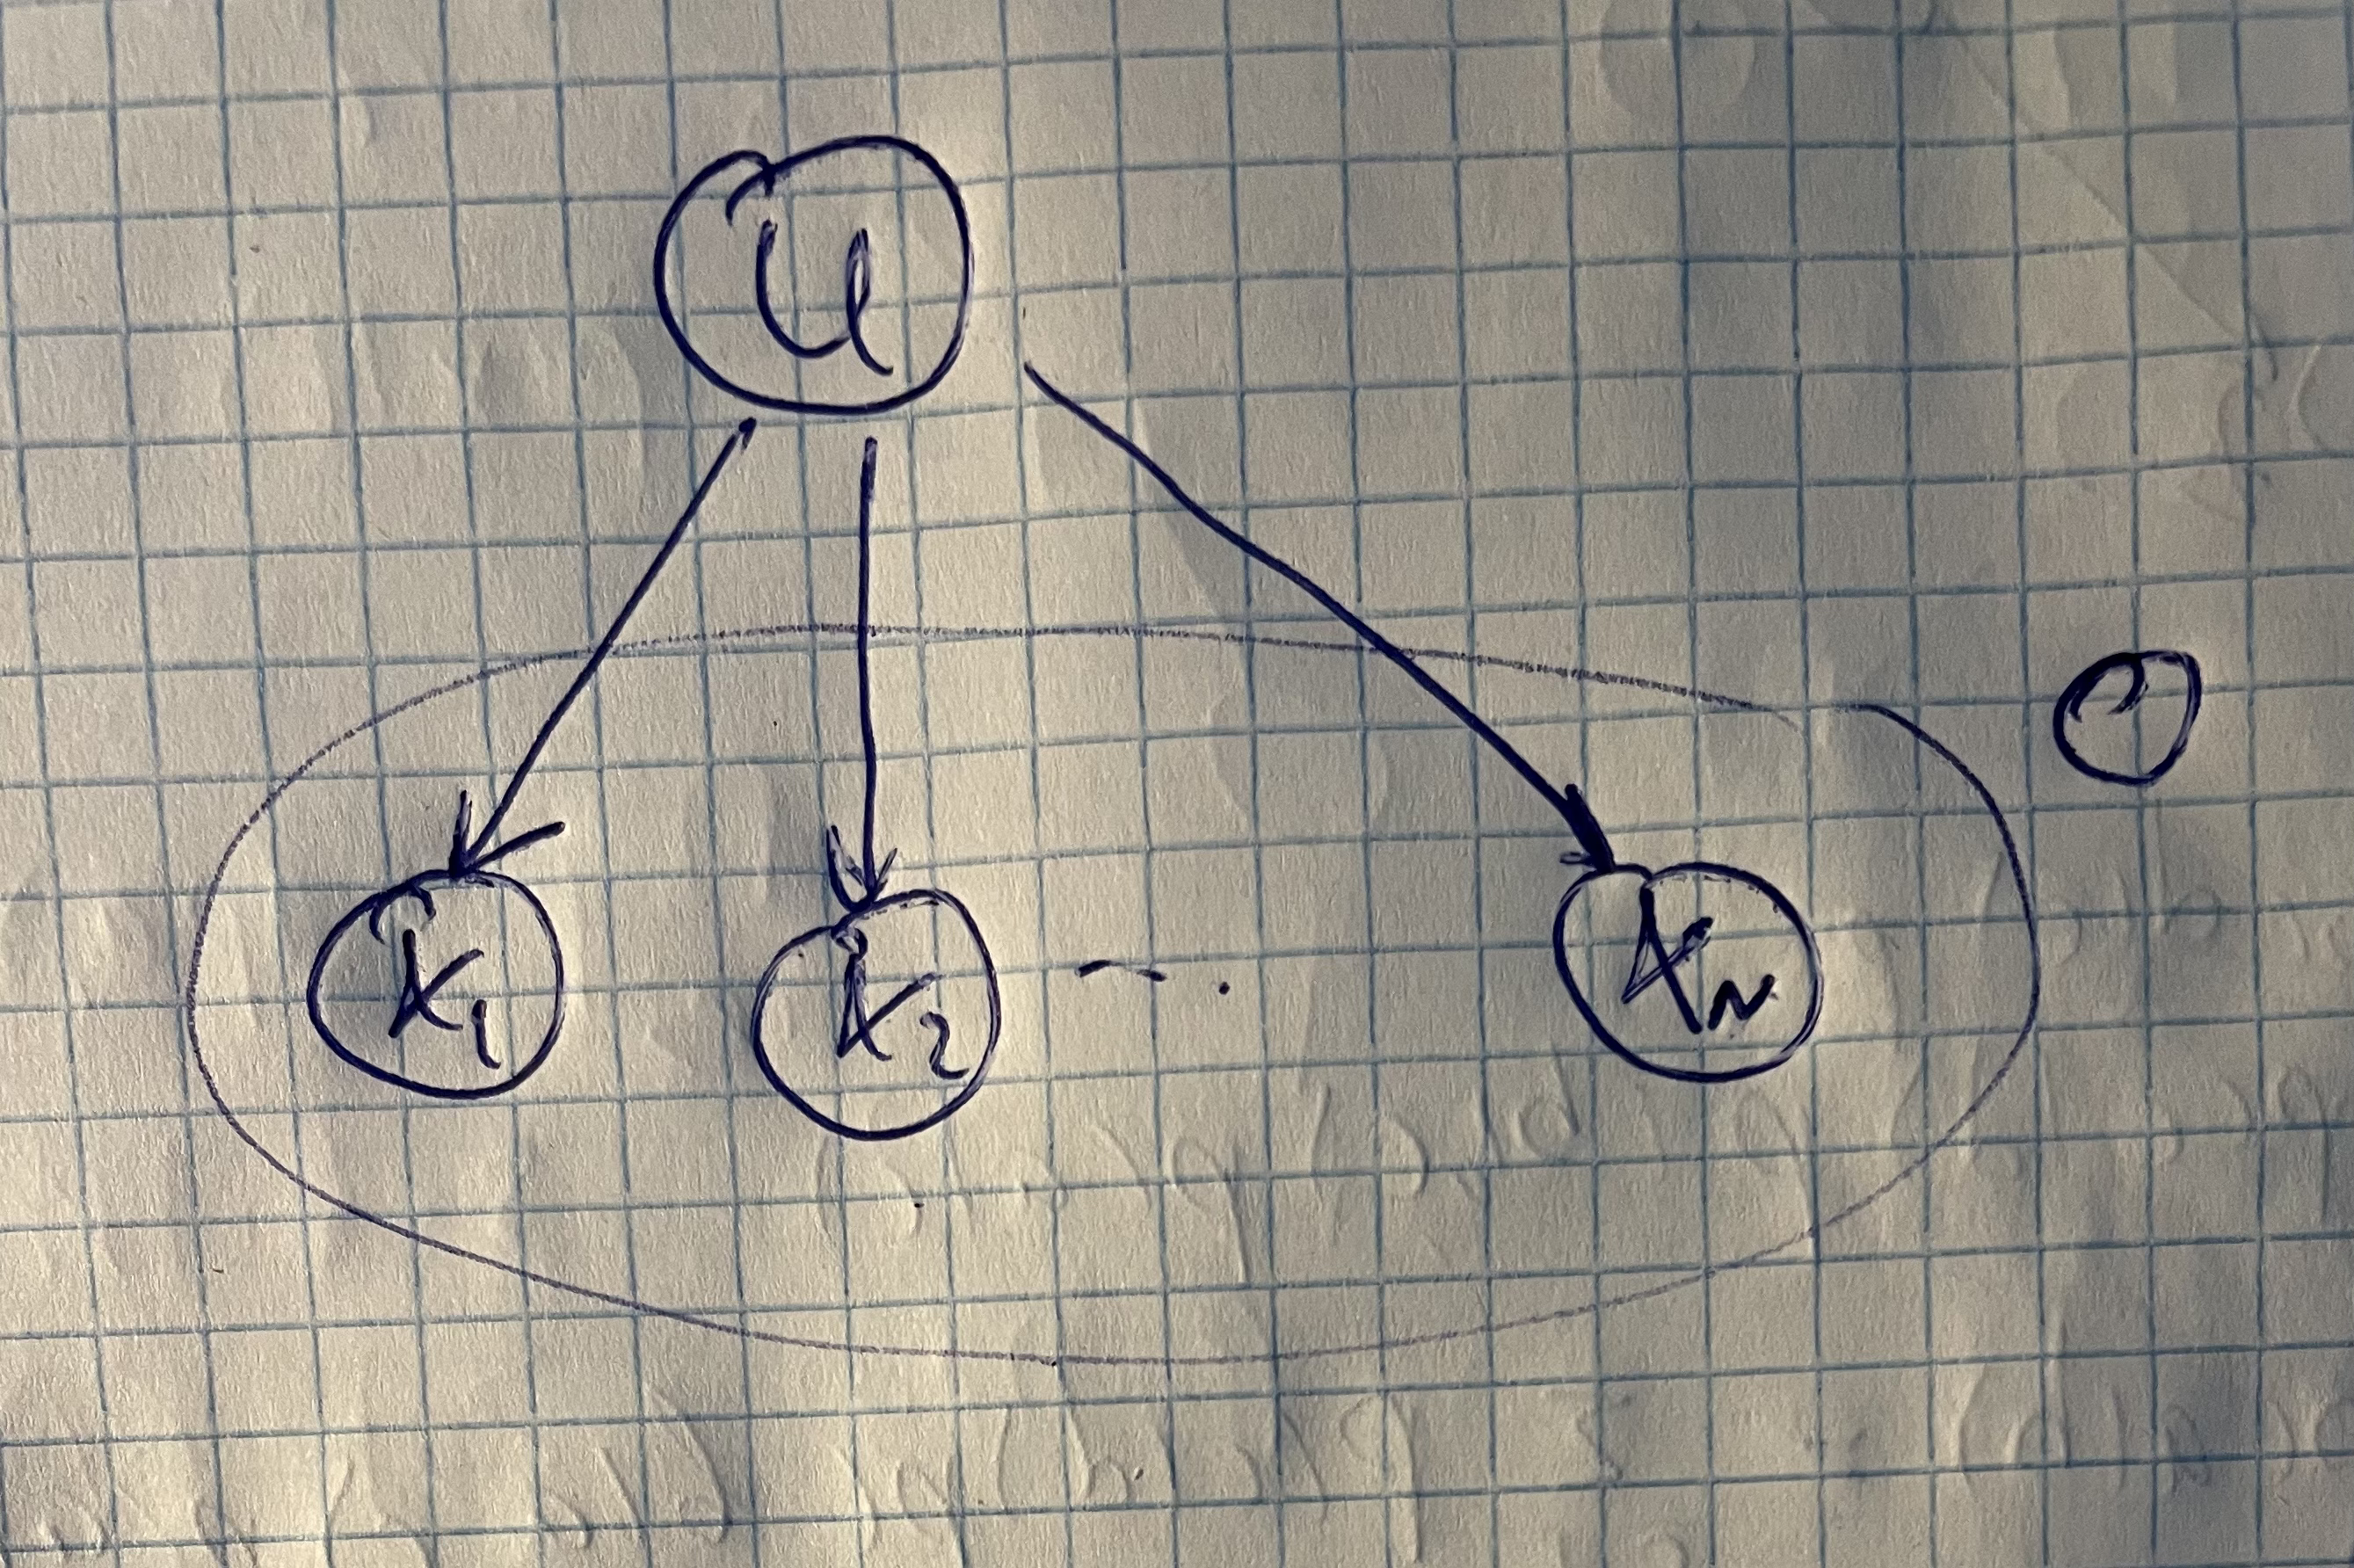
\includegraphics[scale=0.1]{imgs/img2.png}
	\end{center}
	\caption{Довольно бесполезная причинная структура}
	\label{fig:useless_model}
\end{figure}

Идея выбора модели состоит в том, чтобы в некотором смысле она была наиболее простой/минимальной относительно тех данных, которые наблюдаемы.

Дальше введем не совсем формальное пока-что определение выведенной причинности (пока полагаем, что все переменные наблюдаемые)

\define{Выведенная причинность (предв.)} Переменная $X$ имеет причинное влияние на переменную $Y$, если существует направленный путь из $X$ в $Y$ в любом минимальной \textbf{причинной} структуре.

\define{Скрытая структура (latent structure)} это пара $L = (D, O)$, где $D$ - причинная структура над $V$, $O \subset V$ - множество наблюдаемых переменных.

\define{Предпочтение структуры (structure preference)} структура $L = (D, O)$ предпочтительнее структуры $L' = (D', O')$ (пишут $L \preceq L'$) если $D'$ эквивалентно $D$ на множестве наблюдаемых переменных $O$, т.е. тогда и только тогда, когда  $\forall \Theta_D \  \exists \Theta_{D'} : P_{[O]}((D', \Theta_{D'})) = P_{[O]}((D, \Theta_{D}))$. 

Латентные структуры называются эквивалентными, если $L \preceq L'$ и $L' \preceq L$. 

\define{Минимальность (minimality)} структуры $L$ относительно класса структур $C$ означает её предпочтительность относительно всех других структур этого класса: $\forall L' \in C \ L \preceq L'$.

\define{Согласованность} латентной структуры $L = (D, O)$ с распределением $\hat P$ над $O$ означает возможность разместить $\hat P$ в данной латентной структуре, то есть что $\exists \Theta_D : P((O, \Theta_D)) = \hat P$.


\define{Выведенная причинность} С данной $\hat P$ над $O$, переменная $X$ имеет причинное влияние на переменную $Y$, если существует направленный путь из $X$ в $Y$ в любой минимальной \textbf{латентной} структуре.

Надо отметить, что экспрессивная мощность латентной структуры тем выше, чем меньше в ней закодировано независимостей между переменными: таким образом, структуры с меньшим числом незавимостей, согласованные с данными, будут менее предпочтительны, чем структуры с большим числом независимостей в причинной структуре.

\subsection*{Стабильные распределения}

Концепция минимальности латентной структуры позволяет корректно и непротиворечиво получать выводы о причинных связях переменных. Однако, это не всегда вычислительно просто - различных конфигураций структур может быть очень много, и проверять каждую из них на минимальность может быть очень дорого. К тому же, вообще говоря, может же оказаться, что настоящий процесс, генерировавший данные, все таки был порожден моделью, отличной от минимальной? Чтобы упростить себе жизнь, предлагается ввести в рассмотрение ещё один принцип, помимо минимальности - принцип стабильности. 

Начнем с небольшого примера. Рассмотрим процесс, в котором есть две честные монетки. Множеством событий будет выпадение монетки $A$, выпадение монетки $B$, и событие $C$ - "монетки выпали одинаковой стороной". нетрудно заметить, что любая пара переменных безусловно независима, но зависима при условии третьей переменной (например, $P(A=1) = P(A=1|B) = 0.5\ \forall B$, но $P(A=1|B=1) =0.5\neq P(A=1|C=1,B=1) = 1$). Таким образом, любая из структур на \ref{fig:choice} допустима с точки зрения данных и является минимальной. В то же время, если чуть пошатать параметры распределения, например сделать $P(A=1) = 0.6, P(A=0)=0.4$, то уже однозначно не подойдет структура, где $C$ и $B$ независимы безусловно, так как будет $P(C=1) = 0.5$, но $P(C=1|B=1) = 0.6$. Аналогично можно пошатать вероятности для второй монетки, сделав её не совсем честной, и отбросить модель, где $A$ и $C$ независимы.

\begin{figure}[h]
	\begin{center}
		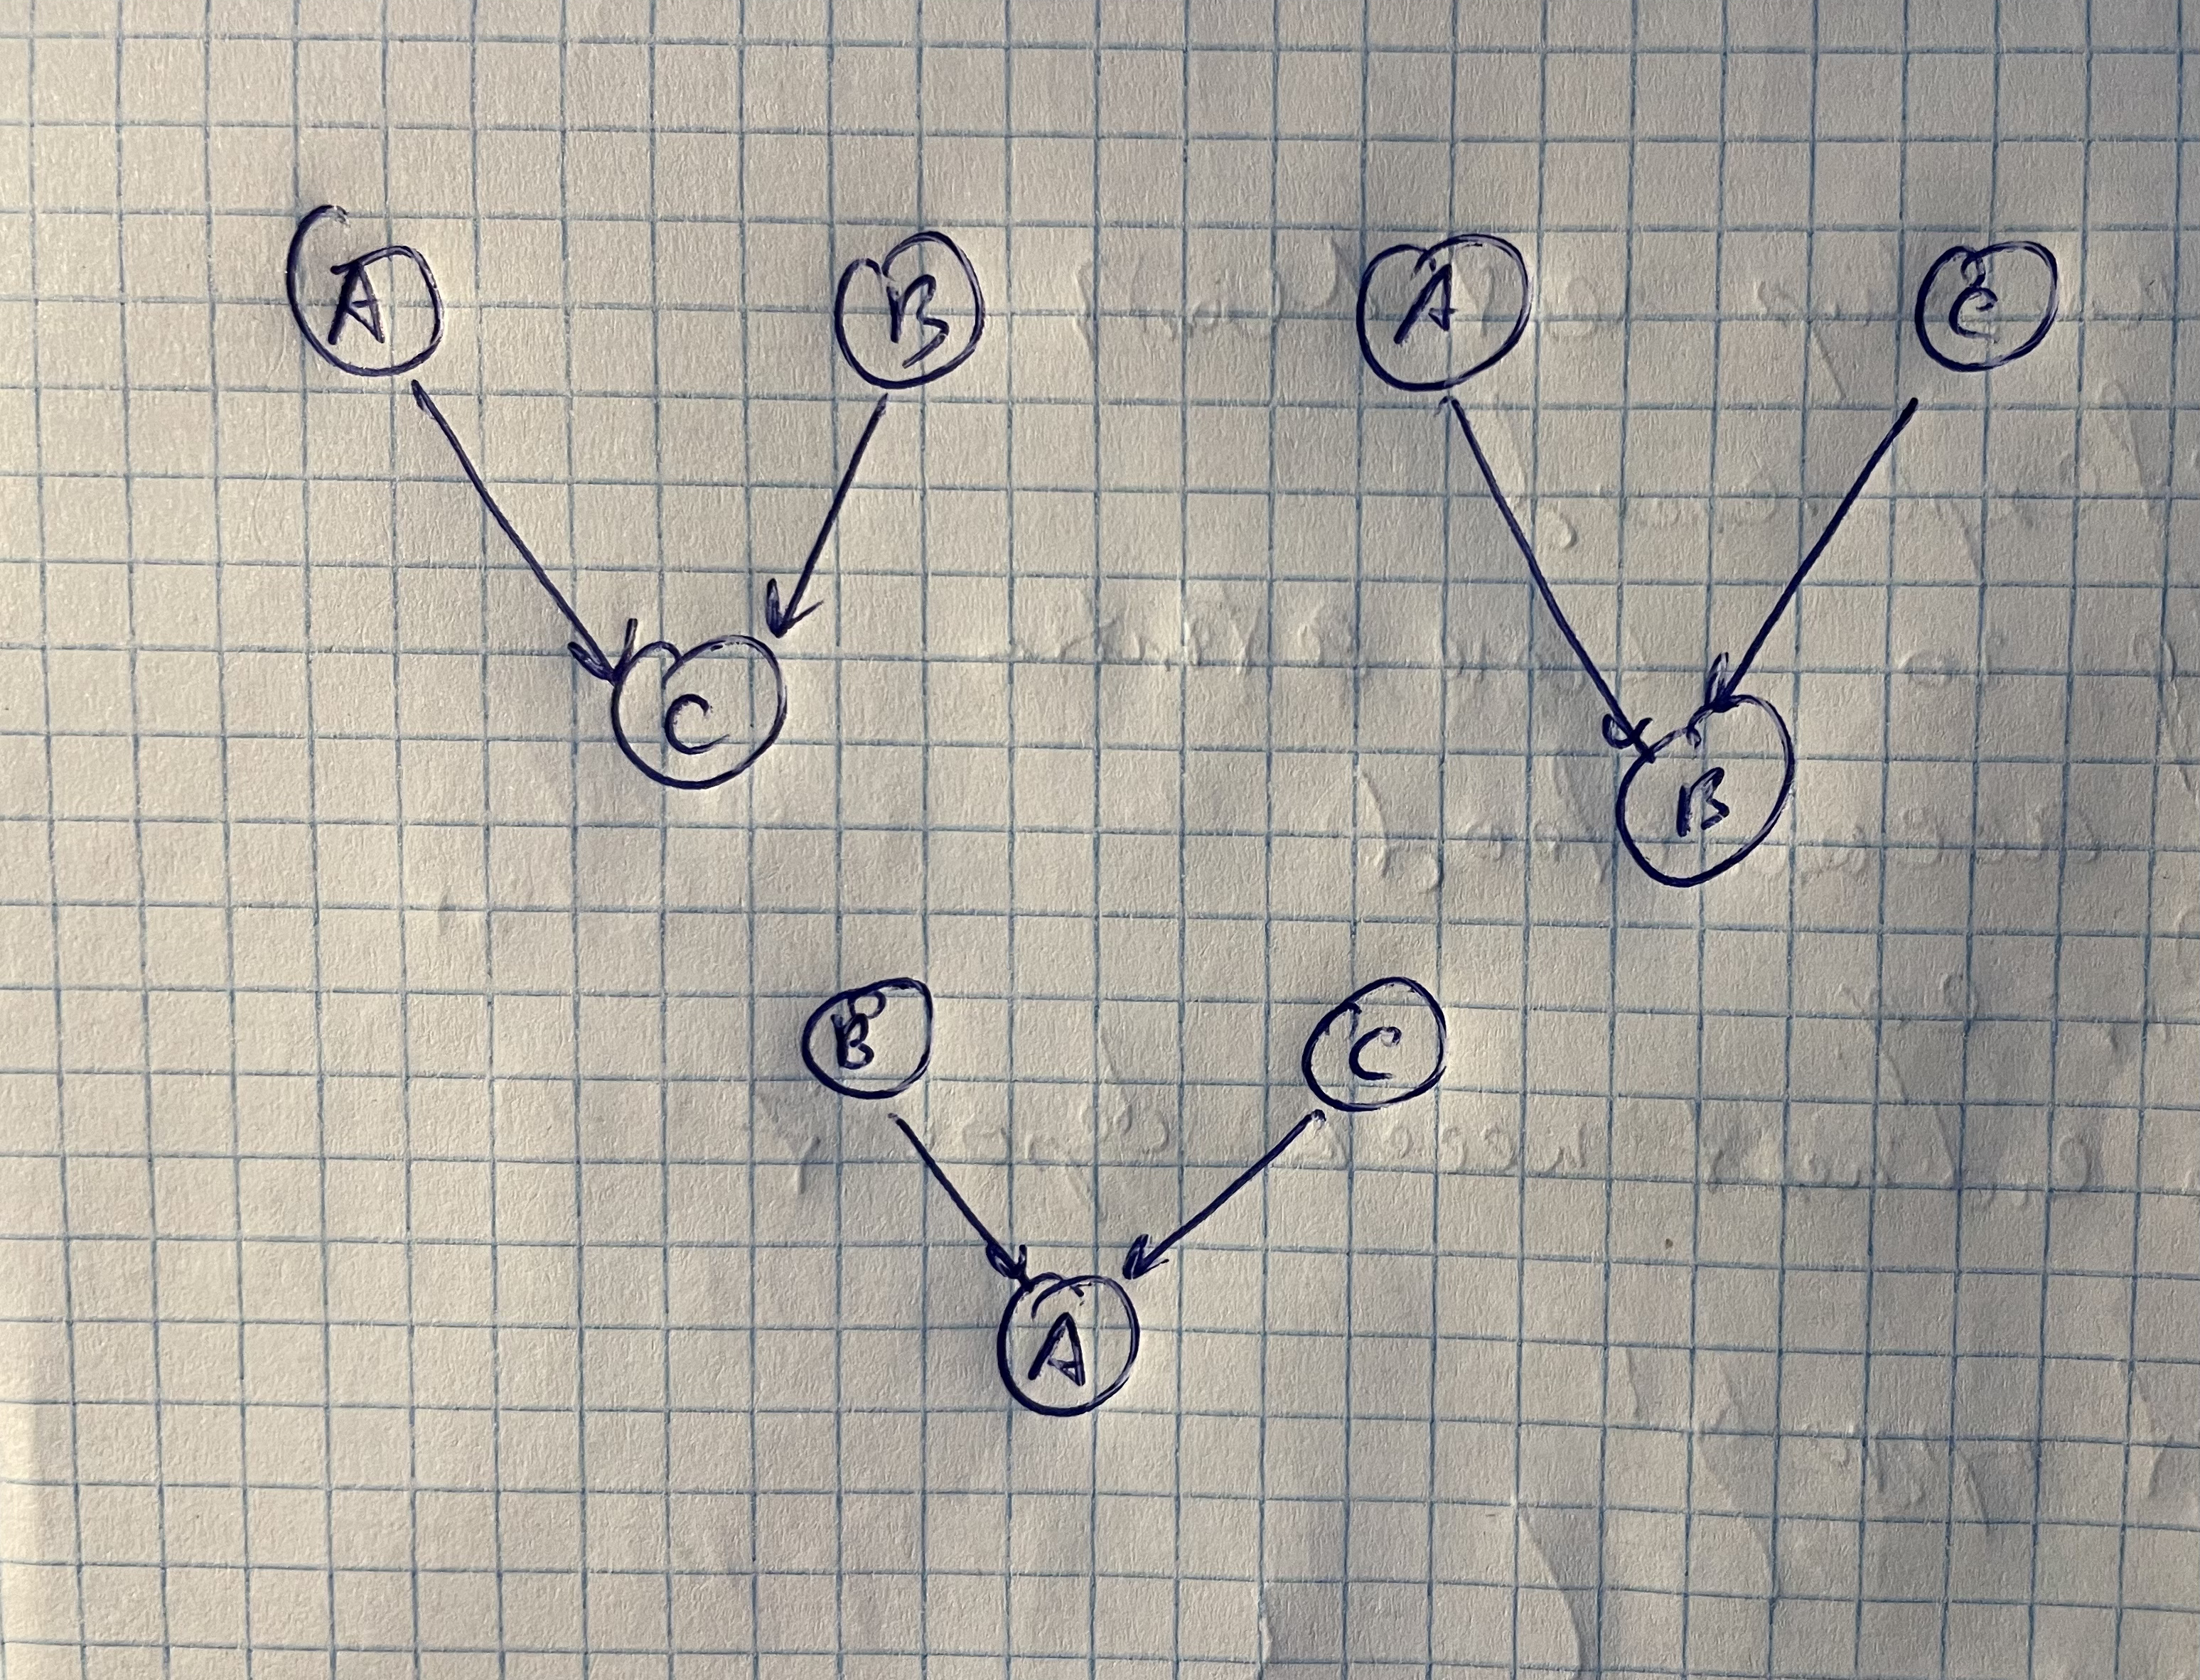
\includegraphics[scale=0.07]{imgs/img3.png}
	\end{center}
	\caption{Какую из трех причинных структур выбрать?}
	\label{fig:choice}
\end{figure}

Для того, чтобы разрулить такие неоднозначности, вводится понятие стабильности:

\define{Стабильность (распределения)} Пусть $I(P)$ - множество всех независимых отношений переменных, заданных через $P$. Причинная модель $M = (D, \Theta_D)$ генерирует стабильное распределение тогда и только тогда когда в $P((D, \Theta_D))$ нет никаких лишних независимостей, т.е. $I(P((D, \Theta_D))) \subset I(P(D, \Theta_{D'}))\ \forall \Theta_{D'}$.

По смыслу, при варьировании параметров от $\Theta$ к $\Theta'$ никакие независимости не должны рушиться, если распределение стабильно. Что пока непонятно - а как выбирать, какие из вероятностей шатать: видимо те которые не ноль? Тогда и правда из стабильности остается только один вариант из трех в приведенном выше примере.

\subsection*{Реконструкция причинной структуры (DAG)}

Когда все переменные наблюдаемы, если использовать принципы минимальности и стабильности, мы всегда будем получать единственную (с точностью до эквивалентности) причинную структуру (эквивалентные структуры - которые шарят одни и те же независимости, то есть один и тот же скелет и v-структуры).

Так как у подлежащей структуры мб эквивалентные, полученный DAG не будет однозначно определяться, поэтому лучшее, что можно сделать - определить его класс эквивалентности. Такой класс эквивалентности называют \textbf{шаблоном} (\textbf{pattern}), и он представляет из себя частично ориентированный граф (ориентируются только те рёбра, которые одинаково направлены во всех графах данного класса эквивалентности).

\textbf{IC (Inductive Causation) Algorithm}

\textbf{Вход:} $\hat P$ - стабильное распределение над переменными $V$.

\textbf{Выход:} $H(\hat P)$ - шаблон, согласованный с $\hat P$.

\textbf{Шаг 1:} Строится неоринетированный граф $D$ на вершинах $V$. Ребром соединяются любые две вершины $a, b$ такие, что $\not\exists S_{ab} \subset V \backslash \{a,b\}:\ a \independent b | S_{ab}$ 

\textbf{Шаг 2:}  $\forall a, b \in V: (a,c) \not \in E$ перебираются их общие соседи $c: (a,c)\in E,  (b,c) \in E$ и проверяется, $c \in S_{ab}$ или нет: если нет, рёбра $a,c$ и $b,c$ ориентируются в сторону $c$ (то есть создаёется новая $v-$структура).

\textbf{Шаг 3:} Ориентируем оставшиеся рёбра, если это можно сделать однозначно при условии, что надо соблюсти условия \begin{itemize}
	\item ацикличности
	\item не добавления новых $v-$структур
\end{itemize}
\end{document}